%\documentclass[landscape,a0paper,fontscale=0.285]{baposter} % a0 is 841mm x 1189mm
\documentclass[landscape,archE,fontscale=0.285]{baposter} % archE is 36in x 48in

% Define colors from UT web page
\selectcolormodel{RGB}
%\definecolor{utburntorange}{cmyk}{0,0.2549,0.3922,0.03529}
\definecolor{burntorange}{RGB}{191,87,0}
\definecolor{rightfooterorange}{RGB}{248,151,31}
\definecolor{pms432}{RGB}{51,63,72}
\definecolor{pms7469}{RGB}{0,95,134}
\definecolor{pms7572}{RGB}{214,210,196}
\definecolor{pms7543}{RGB}{156,173,183}


\usepackage{graphicx} % Required for including images
\graphicspath{{../fig}}

\usepackage{graphbox}
\usepackage{overpic}
\usepackage[caption=false]{subfig}

\usepackage{hyperref}
\hypersetup{
  colorlinks=true,
  urlcolor=pms432,
  pdftitle={Pecos Poster Template},
}

\usepackage{listings}
\lstset{numbers=left,
  basicstyle=\tiny\ttfamily,
  keywordstyle=\color{blue},
  breaklines=true,
  showtabs=false,
  showstringspaces=false,
  xleftmargin=2.5em,
}

\usepackage{amsmath} % For typesetting math
\usepackage{amssymb} % Adds new symbols to be used in math mode

\usepackage{booktabs} % Top and bottom rules for tables
\usepackage{enumitem} % Used to reduce itemize/enumerate spacing
\usepackage{palatino} % Use the Palatino font
\usepackage[font=small,labelfont=bf]{caption} % Required for specifying captions to tables and figures

\usepackage{multicol} % Required for multiple columns
\setlength{\columnsep}{1.5em} % Slightly increase the space between columns
\setlength{\columnseprule}{0mm} % No horizontal rule between columns

\usepackage{tikz} % Required for flow chart
\usetikzlibrary{shapes,arrows} % Tikz libraries required for the flow chart in the template

\newcommand{\compresslist}{ % Define a command to reduce spacing within itemize/enumerate environments, this is used right after \begin{itemize} or \begin{enumerate}
\setlength{\itemsep}{1pt}
\setlength{\parskip}{0pt}
\setlength{\parsep}{0pt}
}
\newcommand{\overbar}[1]{\mkern 1.5mu\overline{\mkern-1.5mu#1\mkern-1.5mu}\mkern 1.5mu}
\newcommand{\pp}[2]{\frac{\partial #1}{\partial #2}}
\newcommand{\dd}[2]{\frac{d #1}{d #2}}
\newcommand{\DD}[2]{\frac{D #1}{D #2}}
\newcommand{\mm}{\mathbf{minmod}}
\def\etal{{\it et al~}}
\newcommand{\be}{\begin{eqnarray}}
	\newcommand{\ee}{\end{eqnarray}}
\newcommand{\mbb}[1]{\mathbb{#1}} % math blackboard bold
\newcommand{\mcal}[1]{\mathcal{#1}} % math blackboard bold
\newcommand{\mbf}[1]{\mathbf{#1}} % math bold face (for vectors)
\newcommand{\sbf}[1]{\boldsymbol{#1}} % bold face for symbols
\newcommand{\jump}[1]{\llbracket #1 \rrbracket} % jump operator
\newcommand{\avg}[1]{\langle #1 \rangle} % average operator
\newcommand{\rarrow}{\rightarrow}
\newcommand{\Rarrow}{\Rightarrow}
\newcommand{\LRarrow}{\Leftrightarrow}
\newcommand{\vvvert}{|\kern-1pt|\kern-1pt|}
\newcommand{\enorm}[1]{\vvvert #1 \vvvert}
\newcommand{\nutil}{\tilde{\nu}}
\newcommand{\Var}{\mathrm{Var}}
\newcommand{\Cov}{\mathrm{Cov}}


\definecolor{MyDarkGreen}{rgb}{0,0.45,0.08}
\newcommand{\myred}[1]{{\color{red} #1}}
\newcommand{\myblue}[1]{{\color{blue} #1}}
\newcommand{\mygreen}[1]{{\color{MyDarkGreen} #1}}

\newcommand{\sa}{\nu_{\mathrm{sa}}}
\newcommand{\tep}{\tilde{\epsilon}}
\newcommand{\Ssd}{\mathcal{S}} % source term due to slow derivative
\newcommand{\ud}{\,\mathrm{d}}

\newcommand{\Mach}[1]{\ensuremath{\mbox{Ma}_{#1}}}
\newcommand{\Reynolds}{\ensuremath{\mathit{Re}}}
\newcommand{\DensityRat}{\ensuremath{\mathit{DR}}}
\newcommand{\BlowRat}{\ensuremath{\mbox{BR}}}
\newcommand{\VelRat}{\ensuremath{\mathit{VR}}}
\newcommand{\Tau}{\ensuremath{\mathrm{T}}}

\newcommand{\wall}     {\ensuremath{\mathrm{w}}}   % wall subindex
\newcommand{\awall}    {\ensuremath{\mathrm{aw}}}  % adiabatic wall subindex

\newcommand{\commentout}[1]{}

\newcommand{\vect}[1]{\boldsymbol{#1}}
\usepackage{mleftright}
\newcommand{\of}[1]{\mleft( #1 \mright)}
\newcommand{\vth}{v_{\textrm{th}}}
\newcommand{\reals}{\mathbb{R}}
\newcommand{\myint}{\int\limits}
\newcommand{\ddt}[1]{\partial_t #1}
\newcommand{\RR}{\mathbb{R}}
\newcommand{\vr}{v}
\newcommand{\diff}[1]{\, d#1}
\newcommand{\norm}[1]{\left\lVert#1\right\rVert}
%\newcommand{\vtheta}{\theta_{\vect{v}}}
%\newcommand{\vphi}{\varphi_{\vect{v}}}
%\newcommand{\vr}{v_{r}}
\newcommand{\vtheta}{{v_{\theta}}}
\newcommand{\vphi}{v_{\varphi}}
\newcommand{\vomega}{v_{\omega}}
\newcommand{\vrunit}{\hat{\vect{v}}_{r}}
\newcommand{\vthetaunit}{\hat{\vect{v}}_{\theta}}
\newcommand{\vphiunit}{\hat{\vect{v}}_{\varphi}}
\DeclareMathOperator{\variance}{Var}


\begin{document}

\begin{poster}
{
columns=4, % number of columns (change to suite your needs)
headerborder=closed, % Adds a border around the header of content boxes
colspacing=1em, % Column spacing
bgColorOne=white, % Background color for the gradient on the left side of the poster
bgColorTwo=white, % Background color for the gradient on the right side of the poster
borderColor=burntorange, % Border color
headershade=plain,
headerColorOne=burntorange, % Background color for the header in the content boxes (left side)
headerColorTwo=burntorange, %burntorange, % Background color for the header in the content boxes (right side)
headerFontColor=white, % Text color for the header text in the content boxes
boxColorOne=white, % Background color of the content boxes
textborder=roundedleft, % Format of the border around content boxes, can be: none, bars, coils, triangles, rectangle, rounded, roundedsmall, roundedright or faded
eyecatcher=false, %true, % Set to false for ignoring the left logo in the title and move the title left
headerheight=0.09\textheight, % Height of the header
headershape=roundedright, % Specify the rounded corner in the content box headers, can be: rectangle, small-rounded, roundedright, roundedleft or rounded
headerfont=\Large\bf\textsc, % Large, bold and sans serif font in the headers of content boxes
%textfont={\setlength{\parindent}{1.5em}}, % Uncomment for paragraph indentation
linewidth=2pt % Width of the border lines around content boxes
}
%----------------------------------------------------------------------------------------
% TITLE SECTION (spans whole width)
%----------------------------------------------------------------------------------------
%
{}
{\bf\textsc{Solving the Boltzmann equation for electron kinetics using the Galerkin approach}\vspace{0.01em}} % Poster title
{\textsc{\small Milinda Fernando, Daniil Bochkov, Todd Oliver, Laxminarayan Raja, Philip Varghese, Robert Moser, and George Biros \hspace{12pt} \\The University of Texas at Austin}} % Author names and institution
{\includegraphics[align=c,height=0.09\textheight]{road_map.png}% just figure (must edit fig to add highlight box)
%\raisebox{-0.5\height}{\begin{overpic}[height=0.09\textheight]{pecos_roadmap_tst_1.5.pdf} % figure + highlight box
%    \put(-1,8){\filldraw [semithick, fill=rightfooterorange, fill opacity=0.1, draw=gray, rounded corners] (1.9,1.2) rectangle +(1.15,0.7);}
%\end{overpic}}%
\hspace{12pt} \includegraphics[align=c,height=3em]{psaap3-logo.png}%
\hspace{12pt} \includegraphics[align=c,height=3em]{oden_pecos_2020_wordmark.png}%
}

%----------------------------------------------------------------------------------------
%	OBJECTIVES
%----------------------------------------------------------------------------------------

\headerbox{Objectives}{name=objectives,column=0,row=0}{
\begin{itemize}
	\item \textbf{\textcolor{orange}{Main}}: Develop scalable robust deterministic Boltzmann solver to determine species kinetics properties to enable accurate plasma simulations. 
	\item \textbf{\textcolor{orange}{Representation}}: Identify robust, yet low cost efficient representation of the distribution function $f(t, \vect{v}, \vect{x})$.
	\item \textbf{\textcolor{orange}{Challenges}}: Dimensionality of the problem (6 + 1 dimensions), numerical + HPC challenges.
\end{itemize}
\vspace{0.3em} % When there are two boxes, some whitespace may need to be added if the one on the right has more content
}

%----------------------------------------------------------------------------------------
%	INTRODUCTION
%----------------------------------------------------------------------------------------

\headerbox{Introduction}{name=introduction,column=1,row=0}{
\begin{itemize}
	\item Electron distribution function $f\of{t,\vect{v}, \vect{x}}$ defines the transport and kinetic properties.
	\item Evolution of $f$ is described by the Boltzmann equation.
	\begin{align}
		\footnotesize
		\partial_t f + \vect{v}\cdot \nabla_{\vect{x}} f  - \frac{\vect{E} q}{m} \cdot \nabla_{\vect{v }}f = C_{en}(f) + C_{ee}(f,f)
	\end{align}
	\item Electric field $\vect{E}$ causes acceleration in the v-space, while the collision operators $C_{en}$ and $C_{ee}$ describes the underlying collisions. 
\end{itemize}
}

\headerbox{Methodology}{name=method,column=0,span=2,below=objectives}{ % This block's bottom aligns with the bottom of the conclusion block
	\begin{multicols}{2}
		\subsubsection*{Discretization}
		\begin{itemize}
			\item Weak formulation.\\
			$
			% \displaystyle
			% \quad
			\partial_t f - \frac{\vect{E} q}{m} \cdot \nabla_{\vect{v}}f = C(f)$
			$
			\Rightarrow 
			\partial_t \myint_{R^3} f \phi\of{\vect{v}} \ud \vect{v} = \myint_{R^3} C(f) \phi\of{\vect{v}} \ud \vect{v}$
			$\quad + \myint_{R^3} \of{\frac{\vect{E} q}{m} \cdot \nabla_{\vect{v}} f} \phi(\vect{v}) \ud \vect{v}$
			\item $f$ is approximated as isotropic + anisotropic correction terms.\\
			$
			% \displaystyle
			% \quad 
			f(\vect{v},t) = \sum_{klm} f_{klm} \Phi_k\of{v} Y_{lm}\of{v_\theta, v_\phi}$
			$ 
			% \displaystyle
			% \quad 
			\text{ with }
			\phi_{pqs}\of{\vect{v}} = \underbrace{\Phi_p\of{v}}_{\text{radial basis}} \underbrace{Y_{qs}\of{v_\theta, v_\phi}}_{\tiny\text{sph. harm.}}$
			\item Electron-heavy collision operator $C_{en}$ in weak form \\
			$
			% \displaystyle
			% \quad 
			% \small
			\myint_{R^3} C_{en} \psi\of{\vect{v}} \diff{\vect{v}} \\
			= N \myint_{v} v^3 \sigma\of{v} f\of{v} \delta_{ql}
			\of{\psi\of{v^{\prime}}\delta_{q0} - \psi\of{v}} \diff{v}$
			\item Electron-electron collisions are modeled with Fokker-Plank equation \\
			$
			% \displaystyle
			% \quad 
			% \small
			\myint_{R^3} C_{ee} \psi\of{\vect{v}} \diff{\vect{v}}=
			\int_{\vect{v}} \nabla \psi\of{\vect{v}} \cdot (f \nabla (\kappa_1\Delta^{-1}f) ) \diff{\vect{v}} +\\
			\frac{1}{2} \int_{\vect{v}} H\psi\of{\vect{v}} : \of{f H (\kappa_2\Delta^{-2}f)} \diff{\vect{v}} 
			$ where $H$ denotes the Hessian operator. 
		\end{itemize}
		\subsubsection*{Steady-state solutions}
		\begin{itemize}
			\item Electric field accelerate electrons (adds energy), while collision causes energy loss.
			\columnbreak
			\item The normalized distribution function $\hat{f}\of{\vect{v},t}$ should reach a steady state.
			%\item We can directly solve the above to compute the steady-state solution.\\
			$
			 \displaystyle
			 \quad
			 \partial_t (\hat{f}) = 0 \Rightarrow R(\hat{f}) = 0 \text{ where } R(\hat{f}) =\\
			 \footnotesize
			 -(u^T C_{en} \hat{f}) \hat{f} + (C_{en}+E)\hat{f} + n_e C_{ee}(\hat{f}, \hat{f}) =0
			$
			\item We use Newton type iteration with line-search algorithm for steady state solution
			$
			\Delta\hat{f} = -[J(\hat{f})]^{-1}R(\hat{f}) \text{ where } \\
			J(\hat{f}) = (C_{en} + E) + n_e (C_{ee}(\cdot, \hat{f}) + C_{ee}(\hat{f}, \cdot)) \\
			-2(u^T C_{en} \hat{f})I
			$
		\end{itemize}
		\vspace{-0.6in}
		\subsubsection*{Transient solution}
			$
			\displaystyle
			\quad
			\partial_t (\hat{f}) = (C+E)\hat{f} + n_e C_{ee}(\hat{f}, \hat{f}) -(u^T C_{en} \hat{f}) \hat{f} \\
			\text{ with } u^T \hat{f} =1
			$
			\begin{itemize}
				\item  Let $p = \frac{u}{\norm{u}_2}$ then note that $(I-pp^T)\bar{f} = \bar{f}$. We write, QR factorization of the projection matrix $(I-pp^T) = Q_{n\times (n-1)} R_{(n-1)\times n}$
				\item Let $\hat{f} = f_1 + Q\bar{f}$ such that $u^T f_1 = 1$ and $u^T Q\bar{f}=0$ where $\bar{f}\in \mathcal{R}^{n-1}$.  Let $f_1= \frac{u}{\norm{u}_2^2}$. Note that $\partial_t \hat{f} = \partial_t (f_1 + Q\bar{f} ) = Q\partial_t \bar{f}$ we can write, 
				$
					\partial_t \bar{f} = Q^T(C+E)\hat{f} + n Q^T C_{ee}(\hat{f}, \hat{f}) \\
					- \of{u^T W(\hat{f})} Q^T\hat{f}
				$, where $\bar{f}(0) = Rf(0)$.
			\end{itemize}
	\end{multicols}
}

%----------------------------------------------------------------------------------------
%	REFERENCES
%----------------------------------------------------------------------------------------

% \headerbox{References}{name=references,column=0,above=bottom}{

% \renewcommand{\section}[2]{\vskip 0.05em} % Get rid of the default "References" section title
% \nocite{*} % Insert publications even if they are not cited in the poster
% \small{ % Reduce the font size in this block
% \bibliographystyle{unsrt}
% \bibliography{sample} % Use sample.bib as the bibliography file
% }}

% %----------------------------------------------------------------------------------------
% %	FUTURE RESEARCH
% %----------------------------------------------------------------------------------------
%\headerbox{1D Glow Discharge}{name=glow_discharge,column=2,span=1,row=0}{
%\begin{center}
%	\includegraphics[width=0.7\textwidth]{eye-candy/glow/glow1.png}
%\end{center}
%\subsubsection*{Formulation}
%\footnotesize{
%\begin{align}
%	&\partial_t f + v\cos\of{\vtheta} \partial_z f -\vect{E}\cdot\nabla_v f = C[f] \\
%	&\textcolor{red!80}{f(\vect{v}, 0, t, \vtheta \leq \frac{\pi}{2})	= 0 \text{ and } f(\vect{v}, L, t, \vtheta > \frac{\pi}{2})	= 0}\\
%	&\partial_t n_i + \partial_z \of{\mu_i n_i E\of{z,t} -D_i \partial_z n_i} = N \gamma \myint_{\varepsilon}\myint_{\vect{\omega}} \varepsilon^{1/2} \sigma_i f d\vect{\omega} d\varepsilon \\
%	& \vect{E} = \nabla \of{\Delta^{-1}\frac{e}{\epsilon_0} \of{n_i- n_e}} \text{ , } n_e = \myint_{\vect{v}} f\of{\vect{v}, z, t} \diff{\vect{v}}
%\end{align}}
%\subsubsection*{Discretization}
%\begin{itemize}
%	\item Use method of discrete ordinates in $\vtheta$, $f_{\vtheta_j} = f(v, \vtheta_j, z, t)$
%	\footnote{
%	\begin{align}
%		\partial_t f_{\vtheta_j} + v\cos\of{\vtheta_j} \partial_z f_{\vtheta_j} = P_{\vtheta_j} (C + E) \begin{bmatrix}
%			f_{\vtheta_0}\\
%			\vdots\\
%			f_{\vtheta_{N_\vtheta}}\\
%		\end{bmatrix} ; \\
%		j=1,..., N_{\vtheta} \nonumber
%	\end{align}}
%	\item Use B-splines + spherical basis representation of $f$ in the velocity-space for collision and v-space advection
%	\item Use finite difference method in $z$ direction
%	\item Use method of lines + with explicit time integrator in time
%	\item First order explicit operator splitting for evolving $n_i$ and $\vect{E}$ field equations
%\end{itemize}
%}
%
%\headerbox{Future Work}{name=future_work,column=2,span=1,row=0,below=glow_discharge,above=bottom}{
%	\begin{itemize}
%	\item Add filtering in $\vtheta$ direction
%	\item Supports adaptive discrete ordinates in space
%	\item Integration with PyKokos and Parla
%	\item Revisit radial discretization
%	\begin{itemize}
%		\item DG or finite volume discretization
%	\end{itemize}
%	%\item Artificial diffusion in speed, for stabilization ?
%\end{itemize}
%}


%----------------------------------------------------------------------------------------
%	CONTACT INFORMATION
%----------------------------------------------------------------------------------------

%%% \headerbox{Contact Information}{name=contact,column=3,aligned=references,above=bottom}{ % This block is as tall as the references block
%%% \begin{description}\compresslist
%%% \item[Web] www.university.edu/smithlab
%%% \item[Email] john@smith.com
%%% \end{description}
%%% }

%----------------------------------------------------------------------------------------
%	CONCLUSION
%----------------------------------------------------------------------------------------

\headerbox{Conclusions}{name=conclusions,column=0,span=4,below=method,above=bottom}{ % This block is as tall as the references block
\begin{itemize}
  \item We present an open-source framework to solve the velocity-space Boltzmann equation using Galerkin approach with tabulated cross-section data. Our framework goes beyond the traditional 2-term approximation for the distribution function. We provide efficient robust solvers for steady state and transient solutions. 
  \item \textbf{Future Work} Add 1d3d solver for the plasma tourch simulations as an initial attempt
\end{itemize}
}

%----------------------------------------------------------------------------------------
%	RESULTS 1
%----------------------------------------------------------------------------------------

\headerbox{Results}{name=results_0d3v,column=2,span=2,row=0,above=conclusions}{
	\begin{itemize}
		\item Self-convergence and comparison with Bolsig code (2-term expansion)
	\end{itemize}
	\begin{minipage}{0.4\textwidth}
	\resizebox{\textwidth}{!}{
		\renewcommand{\arraystretch}{1.2}
		\begin{tabular}{|p{1cm}|p{1cm}|c|c|c|c|c|c|}
			\hline
			\multirow{2}{1cm}{\textbf{E/N (Td)}} & \multirow{2}{1cm}{\boldmath$n_e/N$} & \multicolumn{3}{c|}{\textbf{rel. error vs. Bolsig}} & \multicolumn{3}{c|}{\textbf{rel. error (self convergence)}}\\
			% \hline
			% \textbf{Inactive Modes} & \textbf{Description}\\
			\cline{3-8}
			& & \textbf{elastic} & \textbf{ionization} & \textbf{mobility} & \textbf{elastic} & \textbf{ionization} & \textbf{mobility}\\
			%\hhline{~--}
			\hline
			1        & 0.0 & 7.11E-05 &    --	    & 4.10E-05	& 4.61E-12	&   --	    & 2.47E-12 \\
			5        & 0.0 & 4.12E-04 & 3.74E-04	& 2.92E-06	& 3.83E-07	& 3.84E-04	& 5.34E-07 \\
			20       & 0.0 & 5.76E-04 & 3.49E-03	& 2.98E-04	& 2.77E-04	& 9.74E-03	& 1.29E-03 \\
			100      & 0.0 & 1.35E-03 & 2.74E-03	& 4.85E-03	& 2.02E-03	& 4.11E-02	& 6.65E-04 \\
			\hline
			1        & $10^{-3}$ & 9.40E-03	& 4.40E-03	& 7.99E-03	& 8.61E-07	& 3.60E-05	& 6.40E-07 \\
			5        & $10^{-3}$ & 1.52E-02	& 4.12E-03	& 1.83E-04	& 1.66E-07	& 1.42E-06	& 1.31E-07 \\
			20       & $10^{-3}$ & 1.69E-02	& 1.46E-02	& 1.13E-02	& 6.93E-08	& 1.89E-07	& 6.68E-08 \\
			100      & $10^{-3}$ & 9.11E-03	& 1.87E-02	& 1.65E-02	& 1.53E-07	& 2.96E-07	& 2.50E-07 \\
			\hline
			1        & $10^{-2}$ & 4.88E-03	& 1.20E-02	& 9.94E-03	& 6.72E-06	& 1.77E-04	& 5.18E-06 \\
			5        & $10^{-2}$ & 7.85E-03	& 8.73E-03	& 9.56E-03	& 2.73E-07	& 4.87E-06	& 2.07E-07 \\
			20       & $10^{-2}$ & 1.13E-02	& 4.57E-03	& 6.19E-03	& 1.85E-08	& 4.32E-08	& 1.48E-08 \\
			100      & $10^{-2}$ & 1.19E-02	& 9.93E-03	& 7.76E-03	& 2.50E-08	& 3.24E-09	& 2.57E-08 \\
			\hline
			1        & $10^{-1}$ & 1.72E-03	& 8.17E-03	& 5.31E-03	& 4.39E-05	& 6.37E-04	& 4.01E-05 \\
			5        & $10^{-1}$ & 2.42E-03	& 7.80E-03	& 7.74E-03	& 5.49E-06	& 5.91E-05	& 4.79E-06 \\
			20       & $10^{-1}$ & 3.84E-03	& 7.97E-03	& 8.41E-03	& 5.46E-07	& 5.01E-06	& 4.59E-07 \\
			100      & $10^{-1}$ & 4.76E-03	& 9.80E-04	& 1.89E-03	& 3.97E-08	& 2.88E-07	& 3.35E-08 \\
			\hline
	\end{tabular}}
	\end{minipage}
	\begin{minipage}{0.6\textwidth}
		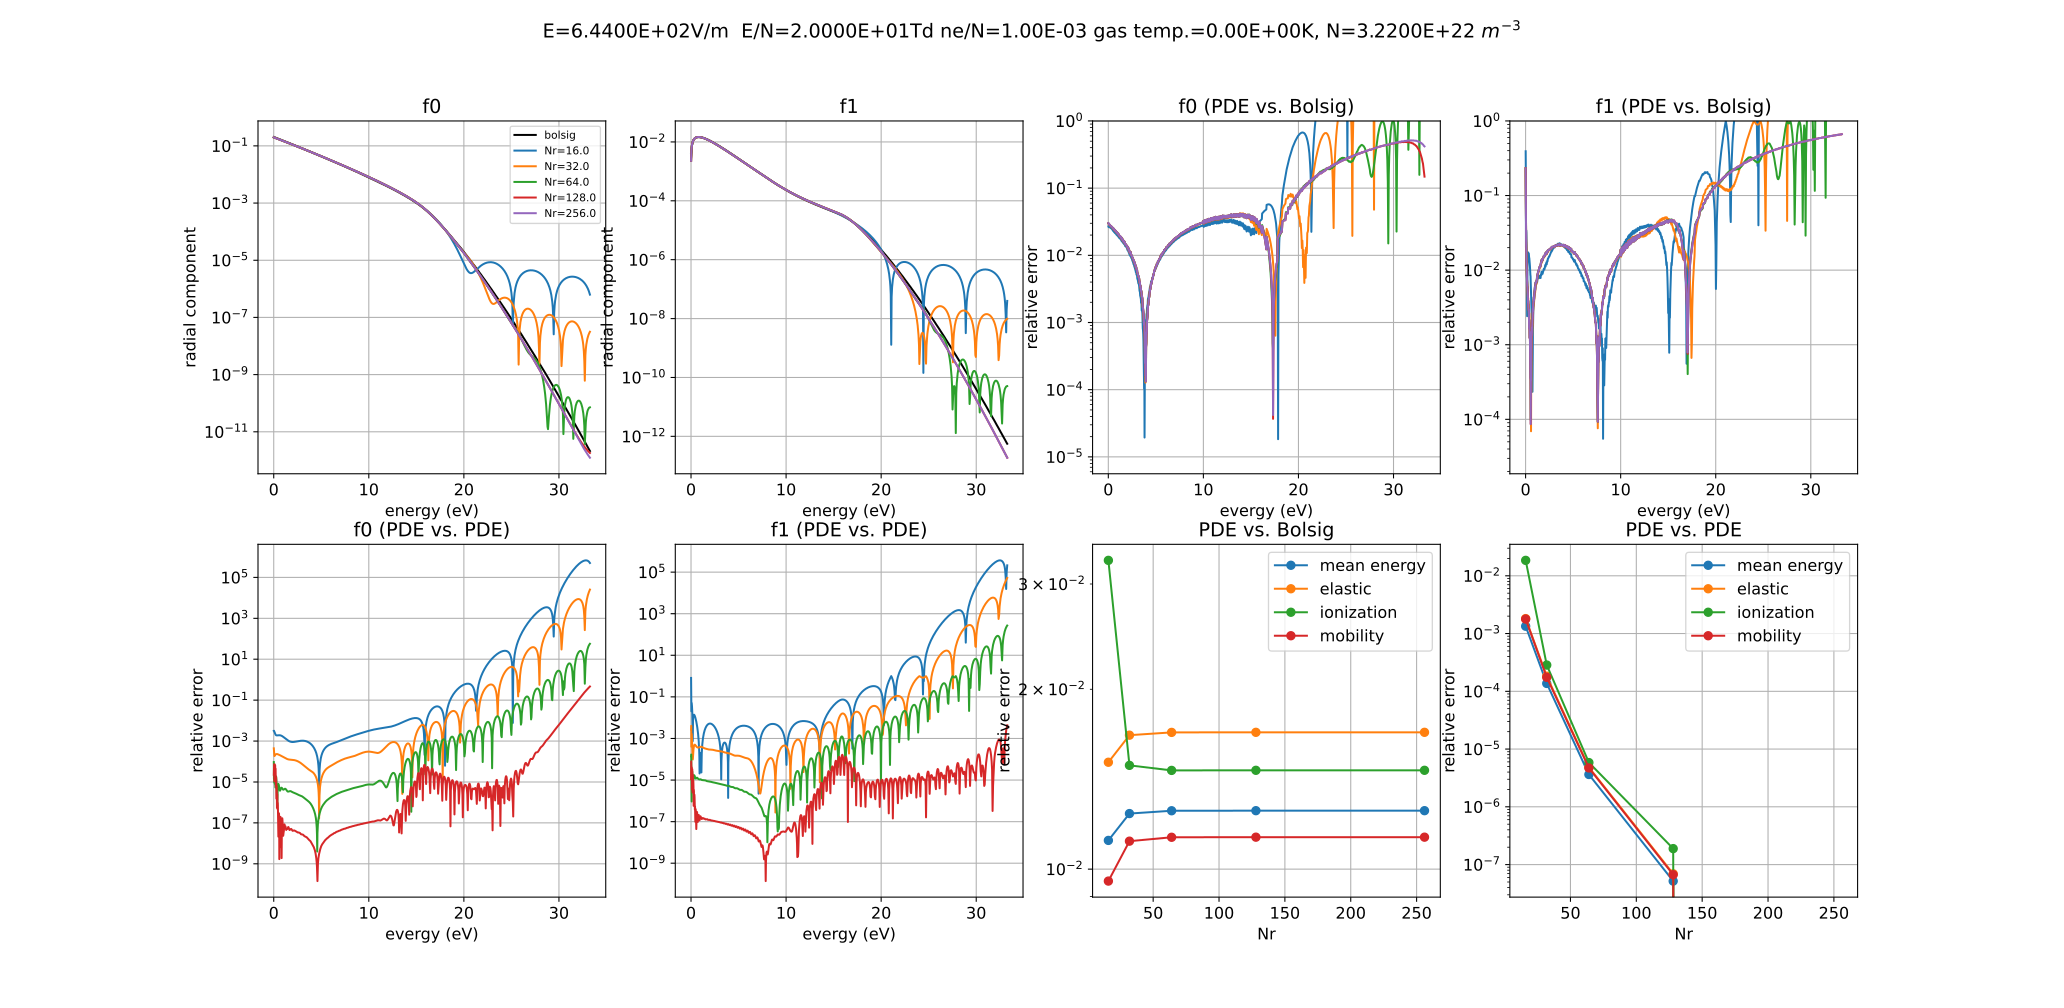
\includegraphics[width=\textwidth]{us_vs_bolsig_cg_g0_g2_E643.9999999999999_poly_bspline_sp_4_nr256_qpn_4_bscale1.0_sweeping_Nr_lmax_1_ion_deg_1.00E-03_Tg0.00E+00.png}
	\end{minipage}
	\begin{itemize}
		\item Effect on electron-electron collisions on the QoIs 
	\end{itemize}
	\begin{minipage}{0.99\textwidth}
		\centering
		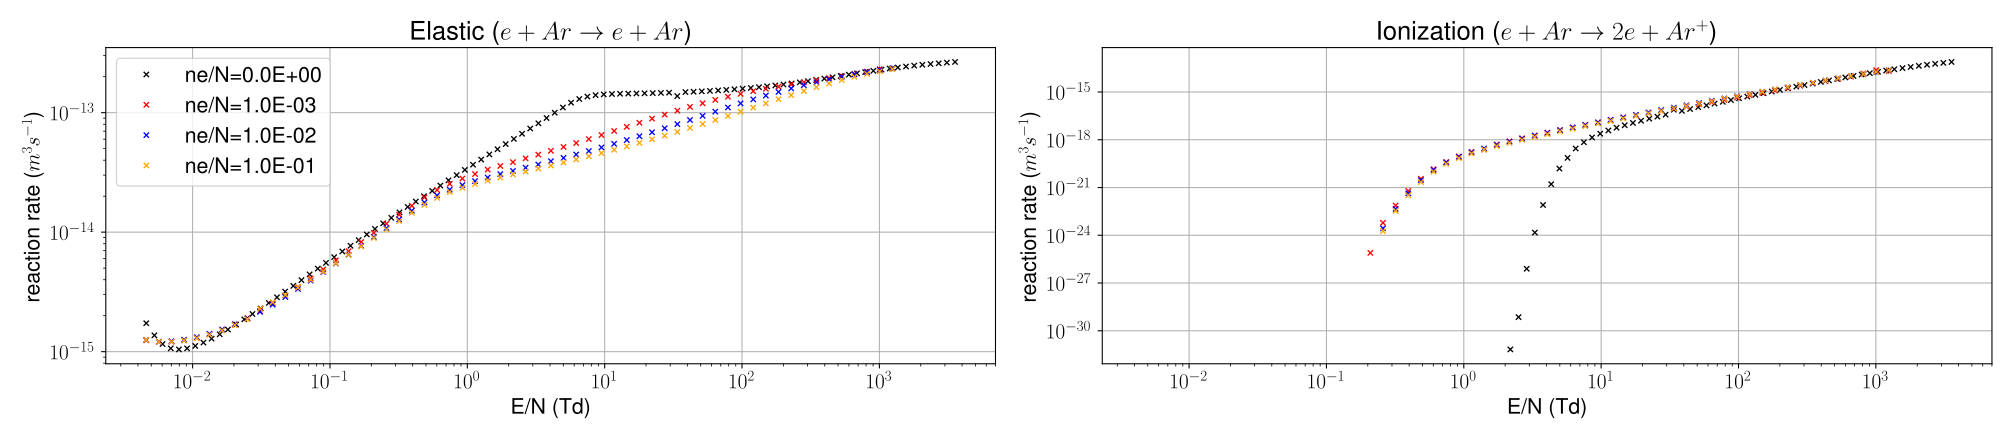
\includegraphics[width=\textwidth]{effect_of_cc.png}
	\end{minipage}
	\begin{center}
	\begin{minipage}{0.83\textwidth}

			\resizebox{\textwidth}{!}{
				\begin{tabular}{cc}
					$E/N=1Td,\ n_e/N = 0$ & $E/N=1Td,\ n_e/N = 1e-3$ \\ 
					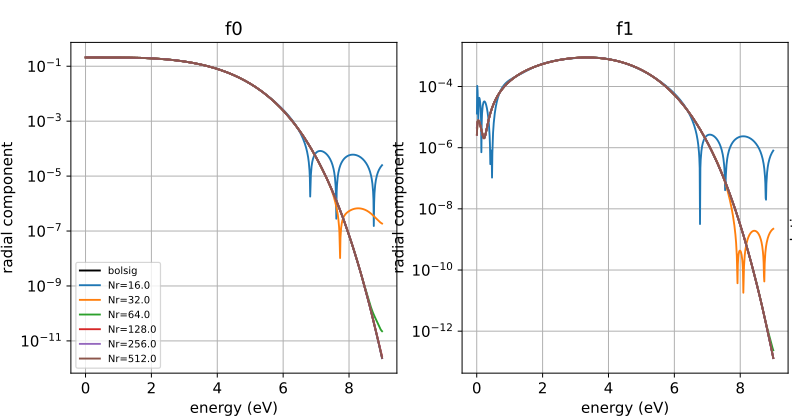
\includegraphics[width=0.48\textwidth]{1TD_ion_deg_0e0.png} & 	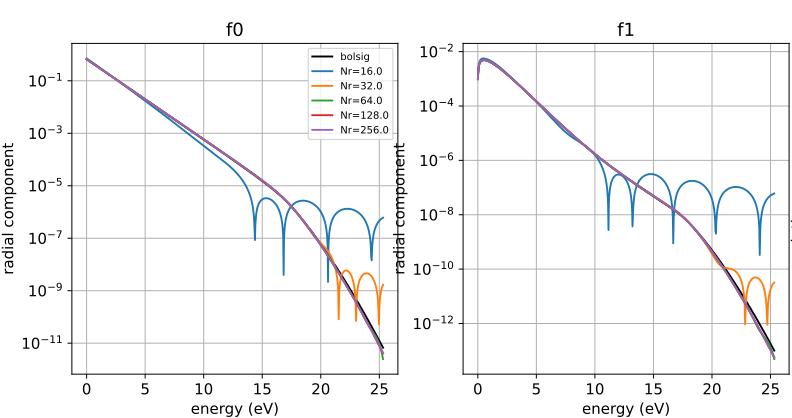
\includegraphics[width=0.48\textwidth]{1TD_ion_deg_1e-3.png}\\
					%		ne/N = 1e-2 & ne/N = 1e-1 \\ 
					%		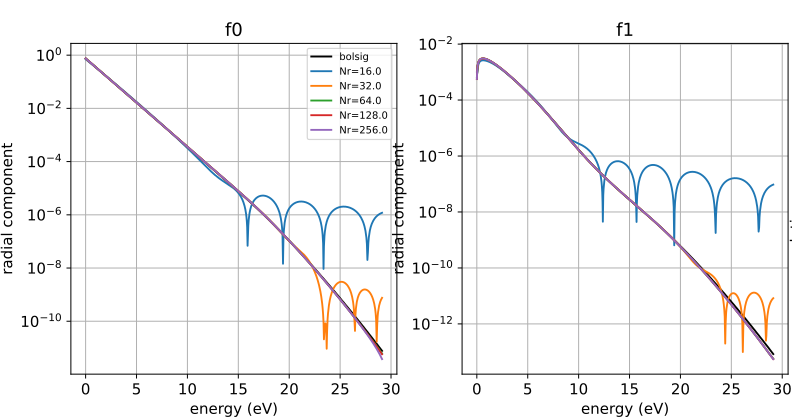
\includegraphics[width=0.48\textwidth]{1TD_ion_deg_1e-2.png} & 	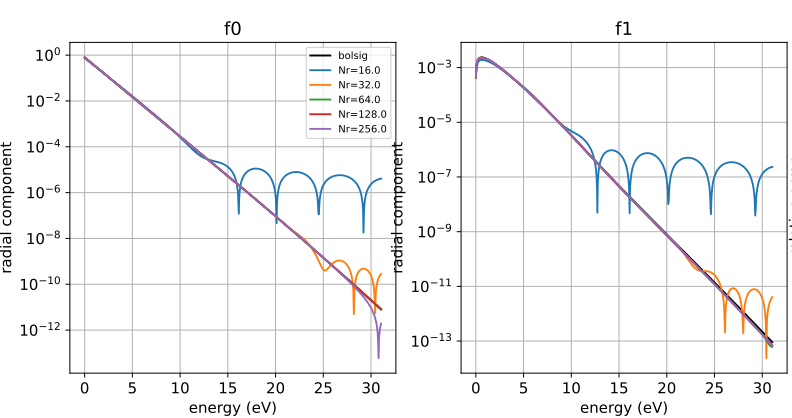
\includegraphics[width=0.48\textwidth]{1TD_ion_deg_1e-1.png}\\
			\end{tabular}}
	\end{minipage}
	\end{center}
	\begin{itemize}
		\item Beyond two-term approximation $E/N = 100Td \text{ and } n_e/N=1e-3$
	\end{itemize}
	\begin{center}
	\begin{minipage}{0.83\textwidth}
		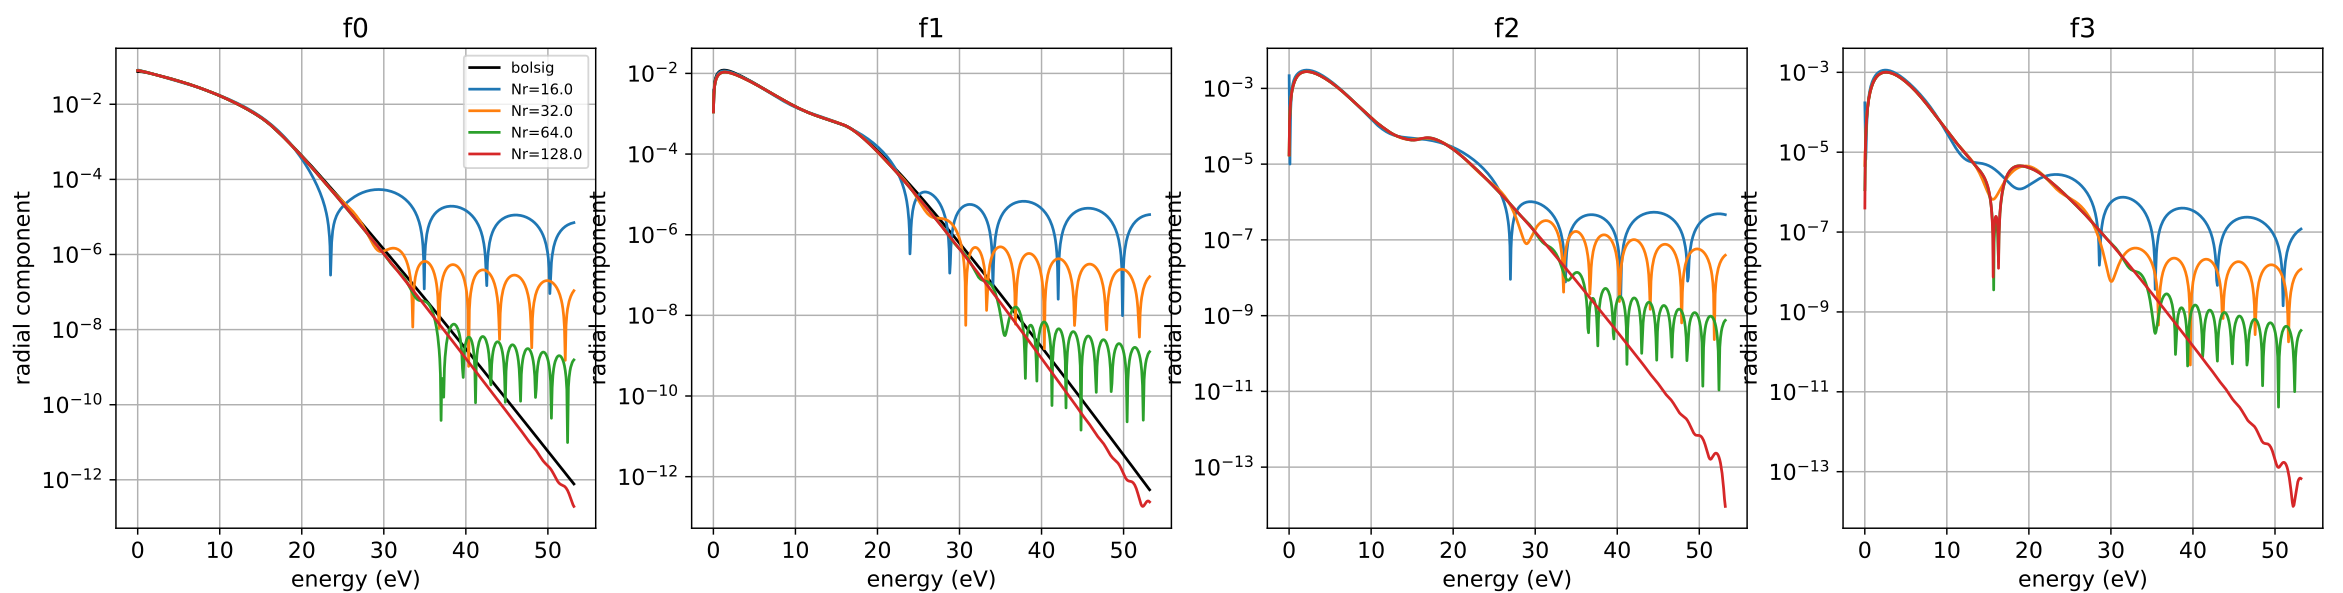
\includegraphics[width=\textwidth]{100Td_ion_deg1e-3.png}
	\end{minipage}
	\end{center}


		%\caption{Deterministic approach self convergence and comparison with the Bolsig code}
%	\subsubsection*{Global vs. Local Galerkin approximations}
%	\begin{center}
%		\includegraphics[width=\textwidth]{maxwell_E200_g0g2.png}
%		\vspace{-0.2in}
%		\captionof{figure}{Maxwell polynomials (global)}
%	\end{center}
%	\vspace{-0.2in}
%	\begin{center}
%		\includegraphics[width=\textwidth]{bspline_sp2_E200_g0g2.png}
%		\vspace{-0.2in}
%		\captionof{figure}{B-Splines (local)}
%	\end{center}
%	\vspace{-0.2in}
%	\begin{center}
%		\includegraphics[width=\textwidth]{bspline_sp2_E200_g0g2_eedf.png}
%		\vspace{-0.2in}
%		\captionof{figure}{B-Splines + EEDF formulation}
%	\end{center}
%	\vspace{-0.2in}
%	\subsubsection*{Validation with Bolsig+ code}
%	\begin{center}
%		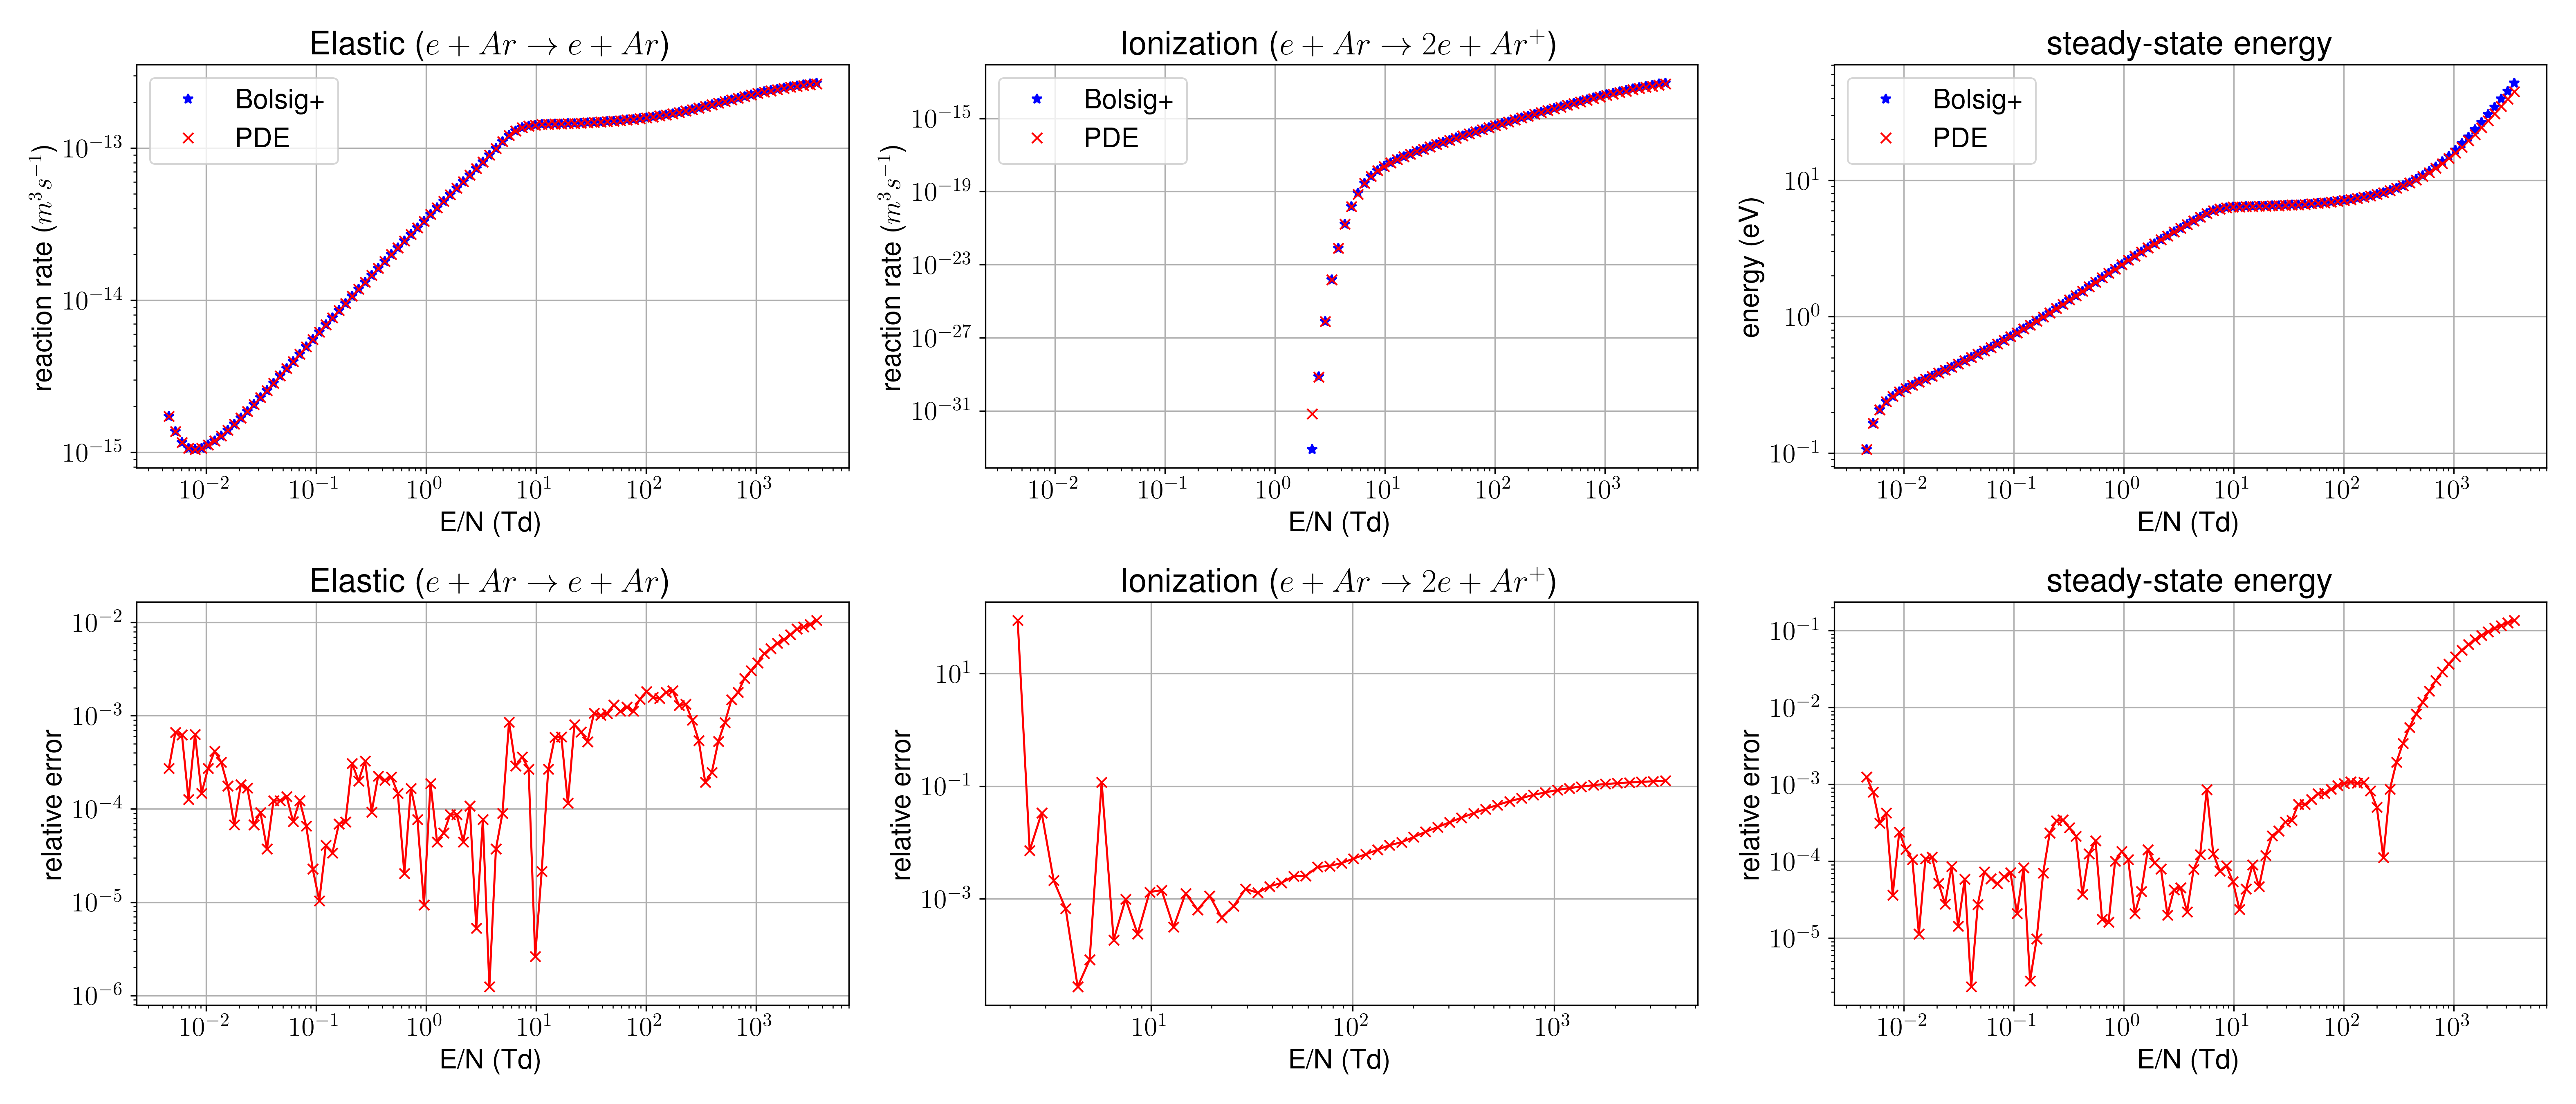
\includegraphics[width=\textwidth]{pde_vs_bolsig_collop_approx_eedf.png}
%		\vspace{-0.2in}
%		\captionof{figure}{Verification results with Bolsig+}
%	\end{center}
}

%\headerbox{Results - 1D3V Boltzmann}{name=results_1d3v,column=3,span=1,row=0,above=bottom,below=results_0d3v}{
%	\subsubsection*{1D Glow Discharge with Boltzmann}
%	\begin{center}
%		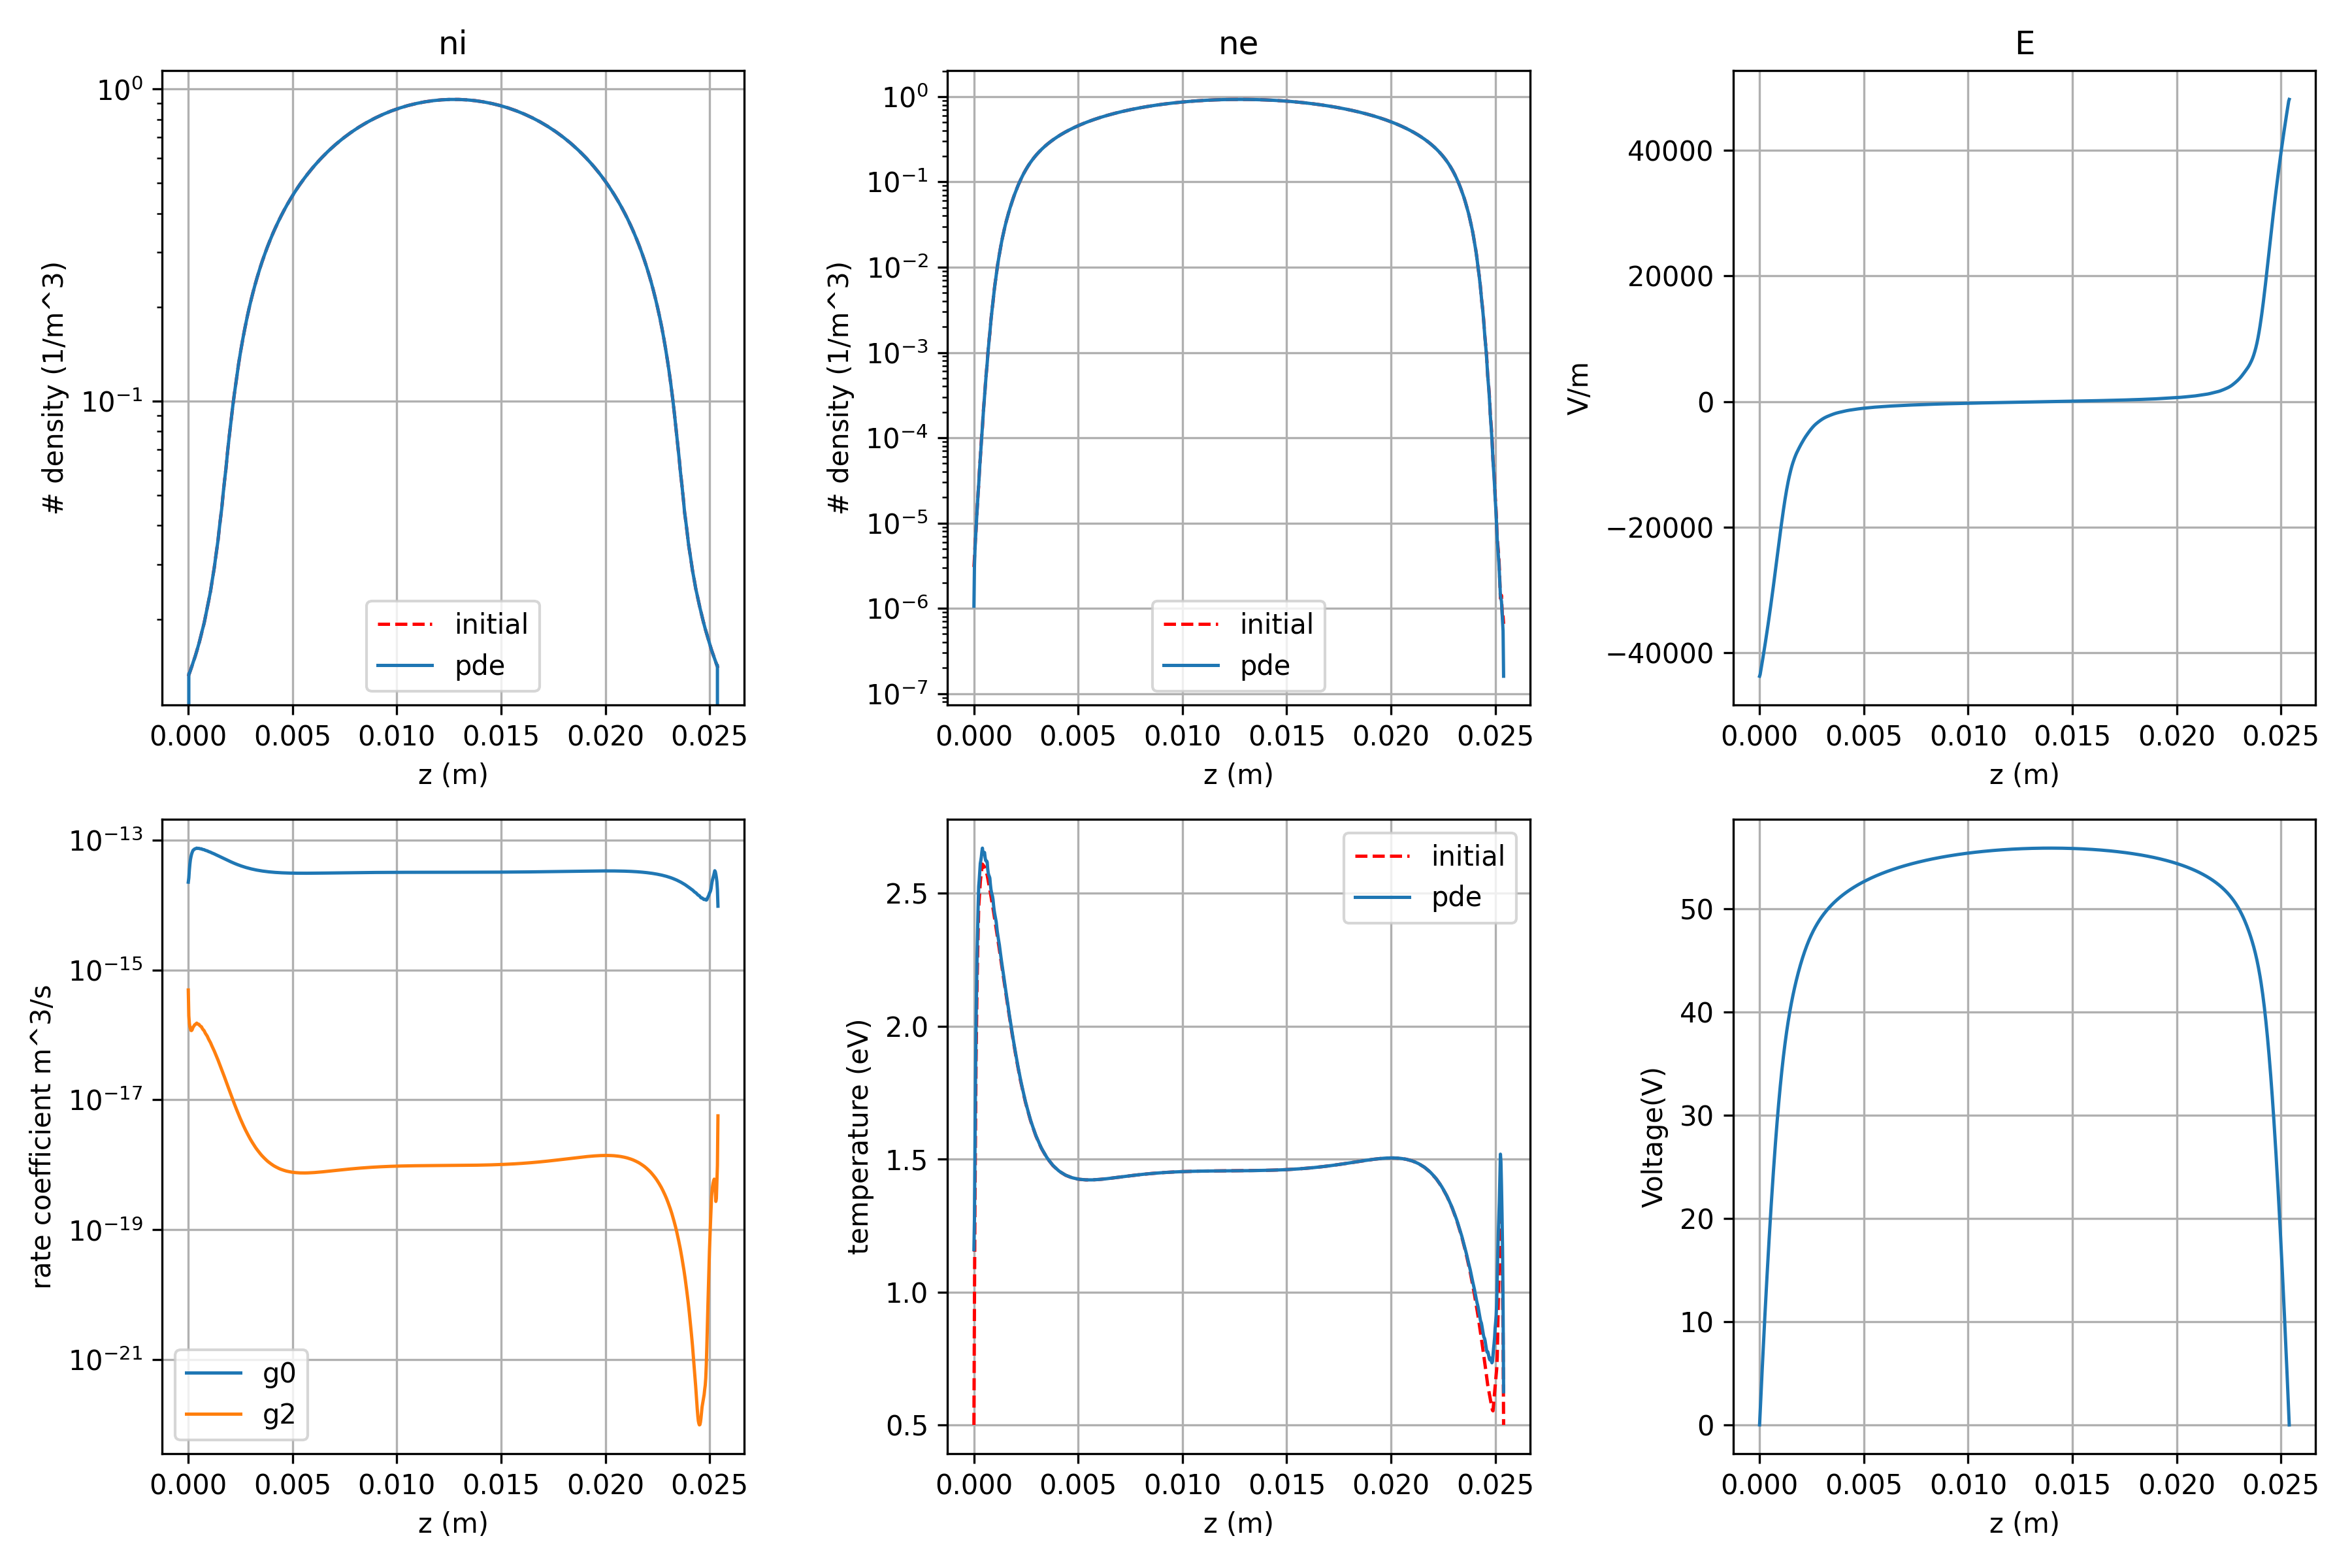
\includegraphics[width=\textwidth]{glow_discharge_1d3v_g0_g2_v0_z01.0_E0.0_poly_bspline_sp_2_nr128_lmax3_qpn4_ev2.000000E+00_bscale1.0_dt1.0000E-13_T1.00E-10_qoi.png}
%		\captionof{figure}{1D glow discharge with Boltzmann equation}
%	\end{center}
%
%}

%----------------------------------------------------------------------------------------
%	MATERIALS AND METHODS
%----------------------------------------------------------------------------------------



%----------------------------------------------------------------------------------------
%	RESULTS 2
%----------------------------------------------------------------------------------------

% \headerbox{Results 2}{name=results2,column=1,below=objectives,bottomaligned=conclusion}{ % This block's bottom aligns with the bottom of the conclusion block

% Donec faucibus purus at tortor egestas eu fermentum dolor facilisis. Maecenas tempor dui eu neque fringilla rutrum. Mauris \emph{lobortis} nisl accumsan.

% \begin{center}
% \begin{tabular}{l l l}
% \toprule
% \textbf{Treatments} & \textbf{Response 1} & \textbf{Response 2}\\
% \midrule
% Treatment 1 & 0.0003262 & 0.562 \\
% Treatment 2 & 0.0015681 & 0.910 \\
% Treatment 3 & 0.0009271 & 0.296 \\
% \bottomrule
% \end{tabular}
% \captionof{table}{Table caption}
% \end{center}

% Nulla ut porttitor enim. Suspendisse venenatis dui eget eros gravida tempor. Mauris feugiat elit et augue placerat ultrices. Morbi accumsan enim nec tortor consectetur non commodo.

% \begin{center}
% \begin{tabular}{l l l}
% \toprule
% \textbf{Treatments} & \textbf{Response 1} & \textbf{Response 2}\\
% \midrule
% Treatment 1 & 0.0003262 & 0.562 \\
% Treatment 2 & 0.0015681 & 0.910 \\
% Treatment 3 & 0.0009271 & 0.296 \\
% \bottomrule
% \end{tabular}
% \captionof{table}{Table caption}
% \end{center}
% }

%----------------------------------------------------------------------------------------

\end{poster}

\end{document}
